\documentclass[11pt]{article}

% ---------------------------------------------------------------
% arXiv-ready source. Compiles with pdflatex + bibtex (TeX Live 2025).
% Figures: figures/*.pdf (vector) and one TikZ figure drawn inline.
% ---------------------------------------------------------------
\usepackage[T1]{fontenc}
\usepackage[utf8]{inputenc}
\usepackage{lmodern}
\usepackage{microtype}
\usepackage[margin=1in]{geometry}
\usepackage{amsmath,amssymb}
\usepackage{graphicx}
\usepackage{booktabs}
\usepackage{tabularx}
\usepackage{array}
\usepackage{enumitem}
\usepackage[section]{placeins}
\usepackage[numbers,sort&compress]{natbib}
\usepackage{xcolor}
\usepackage{tikz}
\usetikzlibrary{arrows.meta,positioning,fit,backgrounds,calc}
\PassOptionsToPackage{hyphens}{url}
\usepackage[hidelinks]{hyperref}
\usepackage{xurl}

\newcolumntype{Y}{>{\raggedright\hskip0pt\emergencystretch=1.5em\arraybackslash}X}
\newcolumntype{P}[1]{>{\raggedright\hskip0pt\emergencystretch=1.5em\arraybackslash}p{#1}}
\newcolumntype{R}{>{\raggedleft\hskip0pt\emergencystretch=1.5em\arraybackslash}X}
\newcolumntype{C}{>{\centering\hskip0pt\emergencystretch=1.5em\arraybackslash}X}
\renewcommand{\arraystretch}{1.15}
\tolerance=1200
\setlength{\emergencystretch}{3em}
\hfuzz=0.5pt
\Urlmuskip=0mu plus 2mu\relax
\expandafter\def\expandafter\UrlBreaks\expandafter{\UrlBreaks\do\-\do\_}
\setlist{itemsep=2pt,topsep=4pt}

\definecolor{accent}{HTML}{2B6CB0}

\newcommand{\KL}{D_{\mathrm{KL}}}

\title{Dual-Plane Agent Transport Over IETF QUIC Streams and Unreliable Datagrams: Eliminating Head-of-Line Blocking in Peer-to-Peer State Sync}

\author{\textbf{Dima Baker}\\
Collective Intelligence Network}

\date{November 2026}

\begin{document}
\maketitle

% ===============================================================
\begin{abstract}
Distributed multi-agent systems increasingly execute parallel tool-invocation graphs and continuous peer-to-peer context synchronization across wide-area networks. However, contemporary agent frameworks encapsulate inter-agent communication inside HTTP/1.1 JSON-RPC or single-connection HTTP/2 gRPC over TCP. Under lossy edge links, TCP enforces strict byte-stream ordering across multiplexed sub-agent tasks, inducing transport-layer Head-of-Line (HoL) blocking where a single dropped packet stalls all concurrent reasoning branches and delays transient state beacons. In this analytical and discrete-event transport simulation study, we formulate multi-agent transport as a dual-plane multiplexed scheduling problem over IETF QUIC (RFC 9000) and Unreliable Datagrams (RFC 9221), and evaluate Dual-Plane QUIC+Datagram. Our architecture separates (1) a Causal Control Plane mapping each sub-agent dependency branch onto an independent QUIC stream with 0-RTT/1-RTT session resumption and strike-register replay protection, from (2) an Ephemeral Telemetry Plane transmitting periodic vector-quantized state beacons over RFC 9221 unreliable datagrams without retransmission stalls. Across 9{,}600 simulated bursts ($N=600$ per cell across $G \in \{2, 4, 8, 16\}$ at $1.5\%$ packet loss and initial congestion window $\mathrm{cwnd}=10$), Dual-Plane QUIC+Datagram achieves $97.83\%$ $[96.33, 98.73]$ sub-65~ms SLO compliance, $16.53$~ms p50 and $69.19$~ms p99 latency, and $16.22$~ms mean beacon Age-of-Information ($7.00\%$ $[5.22, 9.33]$ context drift) at $G=8$, outperforming HTTP/1.1+TCP ($63.00\%$ $[59.07, 66.77]$ SLO, $55.70$~ms p50, $135.89$~ms p99) and gRPC/HTTP2+TCP ($81.17\%$ $[77.84, 84.09]$ SLO, $23.36$~ms p50, $110.16$~ms p99). Both $2\times 2$ payload-vs-transport and Gilbert--Elliott bursty-loss ablations confirm that transport HoL elimination drives the majority of tail-latency reduction.
\end{abstract}

% ===============================================================
\section{Introduction}\label{sec:intro}

As autonomous language model agents transition from single-turn chat interfaces to collaborative, multi-agent execution graphs \citep{arxiv2410_11782, arxiv2507_18224, arxiv2603_19677}, network transport latency has emerged as a primary bottleneck for collective reasoning stability. When an orchestrator agent decomposes a complex task across $G \in [4, 16]$ specialist sub-agents (simultaneously querying code sandboxes, retrieval indices, policy verifiers, and peer state caches) the parent workflow cannot commit its next reasoning step until the critical-path dependency subgraph completes \citep{arxiv2503_13657, elina2026maat}.

\subsection{The transport mismatch in HTTP/TCP agent protocols}

Despite significant research on multi-agent communication topology pruning \citep{zhang2025agentprune, arxiv2410_11782} and latent token compression \citep{arxiv2511_20639}, the underlying network transport layer of production agent protocols (including standard Model Context Protocol deployments and HTTP-based agent-to-agent wrappers) remains anchored to TCP/TLS~1.3 \citep{rescorla2018rfc8446}. Relying on single-socket TCP streams for high-fan-out multi-agent coordination introduces three structural transport pathologies:
\begin{enumerate}
  \item \textbf{Cross-branch Head-of-Line (HoL) blocking in multiplexed TCP.} Even when HTTP/2 (gRPC) multiplexes $G$ logical agent RPCs over a single TCP connection, the operating system kernel treats the connection as a single linearly ordered byte array \citep{langley2017quic, iyengar2021rfc9000}. When a single MTU packet carrying bytes for Sub-Agent~1 is dropped on a wireless or wide-area link with packet loss probability $p_{\mathrm{loss}} \allowbreak \in [0.5\%,\allowbreak 3.0\%]$, the receiving kernel withholds already-arrived packets belonging to Sub-Agents $2, \dots, G$ from the application layer until the TCP retransmission arrives one round-trip time ($\mathrm{RTT}$) later \citep{kuehlewind2022rfc9308}.
  \item \textbf{Handshake round-trip multiplication across ephemeral peer edges.} In decentralized peer-to-peer agent networks where edge nodes dynamically discover and query specialists \citep{ari2018_18, nandakumar2026pace}, establishing a fresh TCP socket followed by a TLS~1.3 handshake incurs 2~full RTTs before the first byte of an agent payload is transmitted (1~RTT for TCP \texttt{SYN}/\texttt{SYN-ACK} plus 1~RTT for TLS~1.3 \texttt{ClientHello}/\texttt{ServerHello}) \citep{rescorla2018rfc8446}.
  \item \textbf{Retransmission-induced Age-of-Information inflation on ephemeral telemetry.} Collaborative agents frequently exchange high-frequency heartbeat beacons, belief-confidence scalars, and speculative KV-cache summaries that are rapidly superseded by newer ticks \citep{rodrigues2026drift, itkin2026delayed}. Transmitting ephemeral state beacons over a reliable, ordered stream forces the transport layer to retransmit dropped obsolete beacons and stall fresh beacons behind them. \citet{rodrigues2026drift} formalize how asynchronous state staleness induces multi-agent context drift, while \citet{itkin2026delayed} prove mathematically that delayed verification updates destabilize multi-agent belief convergence once staleness exceeds a critical stability threshold.
\end{enumerate}

\subsection{IETF QUIC streams, unreliable datagrams, and 2025--2026 protocol developments}

The Internet Engineering Task Force (IETF) QUIC transport protocol (RFC 9000) \citep{iyengar2021rfc9000, langley2017quic} and its Unreliable Datagram Extension (RFC 9221) \citep{pauly2022rfc9221} provide transport-layer primitives specifically engineered to eliminate cross-stream HoL blocking and decouple reliable framing from unreliable real-time datagrams \citep{schinazi2022rfc9297, kuehlewind2022rfc9308}:
\begin{itemize}
  \item \textbf{Per-stream ordered delivery without cross-stream HoL stalls (RFC 9000):} QUIC integrates TLS~1.3 key exchange directly into its UDP transport handshake (achieving 1-RTT cold start and 0-RTT session resumption) and exposes lightweight, independent bidirectional and unidirectional streams \citep{iyengar2021rfc9000, rescorla2018rfc8446}. Packet loss on Stream~$g$ blocks only Stream~$g$; packets arriving for Streams~$g' \neq g$ are decrypted and delivered immediately to the agent runtime \citep{kuehlewind2022rfc9308}.
  \item \textbf{Encrypted, congestion-controlled unreliable datagrams (RFC 9221 \& RFC 9297):} RFC 9221 adds a \texttt{DATAGRAM} frame type to QUIC that shares the connection's authenticated encryption (AEAD), NAT traversal path \citep{ari2018_18}, and congestion controller, but omits retransmission and stream ordering \citep{pauly2022rfc9221, schinazi2022rfc9297}.
  \item \textbf{Emerging 2026 agent and edge transport research:} In the IETF standardization arena, \citet{nandakumar2026pace} submitted an individual Internet-Draft (\texttt{draft-nandakumar-agentproto-pace-00}, Protocol for Agent Communication and Execution) exploring multiplexed transport bindings for agentic workflows. Concurrently, \citet{commey2026matter} quantified post-quantum session establishment fragmentation and transport framing over constrained mesh protocols, \citet{phamtuan2026hpqake} introduced sign-less hybrid post-quantum authenticated key exchange (HPQ-AKE) for bandwidth-constrained edge links, and \citet{buchet2026quicproxies} demonstrated explicit QUIC proxy routing with connection migration. On the security and verification side, \citet{fischlin2024quic} established formal multi-stage security bounds and 0-RTT replay protection requirements for QUIC, \citet{arote2026renegade} showed that cryptographic transport security alone leaves peer-to-peer networks vulnerable to timing and metadata side-channel inference without traffic shaping, and \citet{xiong2026skillguard}, \citet{arxiv2604_11790}, and \citet{elina2026maat} demonstrated deterministic contract and boundary interception for multi-agent tool invocations.
\end{itemize}

\subsection{Contributions}

We formulate, specify, and mechanistically benchmark a dual-plane QUIC transport architecture for peer-to-peer agent state synchronization:
\begin{enumerate}
  \item \textbf{Dual-plane transport taxonomy (Section~\ref{sec:taxonomy}).} We map distinct classes of multi-agent traffic (causal tool RPCs, non-idempotent state commits, ephemeral belief beacons, and store-and-forward bundles) onto their exact IETF transport primitives (Table~\ref{tab:taxonomy}).
  \item \textbf{Queueing, Age-of-Information, and 0-RTT security formulation (Section~\ref{sec:formal}).} We derive (i) the critical-path completion time gap between single-FIFO TCP and $G$-stream QUIC (Equation~\ref{eq:hol_gap}), (ii) the exact renewal-process expected Age of Information $\mathbb{E}[\Delta t_{\mathrm{AoI}}]$ for periodic datagram beacons under geometric packet loss and its Jensen upper bound on Poisson context-drift probability (Equation~\ref{eq:context_drift}), and (iii) the 0-RTT replay-window and hybrid key-exchange budget (Equation~\ref{eq:hybrid_pqc_0rtt}).
  \item \textbf{Dual-Plane QUIC+Datagram architecture and parameter provenance (Section~\ref{sec:architecture}).} We specify the stream-per-branch dispatcher, RFC 9221 datagram beacon scheduler, and idempotency strike register separating the Causal Control Plane from the Ephemeral Telemetry Plane (Figure~\ref{fig:architecture}, Table~\ref{tab:readiness}).
  \item \textbf{Discrete-event simulation, $2\times 2$ payload-vs-transport ablation, and loss-rate sweep (Section~\ref{sec:experiments}).} We execute a discrete-event packet simulator (\texttt{experiment.\linebreak[0]py}) across 9{,}600 multi-agent synchronization bursts ($N=600$ per cell across $G \in \{2,\allowbreak 4,\allowbreak 8,\allowbreak 16\}$), isolating payload compression from transport HoL elimination via a $2\times 2$ factorial ablation at $G=8$ and sweeping packet loss $p_{\mathrm{loss}} \allowbreak \in [0.05\%,\allowbreak 5.0\%]$ (Table~\ref{tab:results}, Figures~\ref{fig:benchmark}--\ref{fig:ablation}).
  \item \textbf{Adversarial transport risks and falsification protocol (Sections~\ref{sec:counter}--\ref{sec:protocol}).} We analyze 0-RTT replay attacks \citep{fischlin2024quic}, traffic-analysis metadata leakage \citep{arote2026renegade}, post-quantum MTU fragmentation \citep{commey2026matter}, and enterprise UDP firewall blackholing \citep{kuehlewind2022rfc9308}, closing with six pre-registerable falsification tests (Table~\ref{tab:protocol}).
\end{enumerate}

% ===============================================================
\section{Multi-agent traffic taxonomy and IETF transport mapping}\label{sec:taxonomy}

Multi-agent frameworks typically treat all network messages as uniform JSON-over-HTTP requests. In practice, agent-to-agent traffic divides into four orthogonal semantic classes with incompatible reliability, ordering, and replay-safety requirements. Table~\ref{tab:taxonomy} maps these four traffic classes onto canonical IETF transport constructs.

\begin{table}[ht]
\centering
\small
\caption{Mapping multi-agent communication classes onto canonical IETF QUIC, TLS 1.3, and DTN transport primitives.}
\label{tab:taxonomy}
\begin{tabularx}{\textwidth}{@{}P{2.2cm}P{2.5cm}P{2.4cm}YP{2.5cm}@{}}
\toprule
Agent traffic class & Canonical primitive & Transport plane & Operational guarantee & Primary grounding \\
\midrule
Read-only parallel sub-agent queries & Independent QUIC streams + 0-RTT tickets & Plane 1: Causal Control Stream ($\mathcal{S}_g$) & Eliminates cross-branch HoL blocking; allows 0-RTT early data for idempotent read queries & \citep{iyengar2021rfc9000, rescorla2018rfc8446, fischlin2024quic, kuehlewind2022rfc9308}\\
State-mutating tool \& contract commits & 1-RTT Forward-Secret QUIC Stream + Strike Register & Plane 1: Authenticated Commit Stream & Forbids 0-RTT early-data replay; enforces Maat/ClawGuard deterministic contract checks & \citep{fischlin2024quic, elina2026maat, arxiv2604_11790, xiong2026skillguard} \\
Periodic context \& heartbeat beacons & QUIC Unreliable Datagrams (RFC 9221 / RFC 9297) & Plane 2: Ephemeral Telemetry Plane ($\mathcal{D}_u$) & Congestion-controlled, AEAD-encrypted fire-and-forget delivery; zero retransmission HoL stall & \citep{pauly2022rfc9221, schinazi2022rfc9297, rodrigues2026drift, itkin2026delayed}\\
Disconnected / intermittent edge bundles & DTN Bundle Protocol v7 + MLS Group Epoch Keys & Store-and-forward overlay & Custodial bundle persistence across intermittent links with RFC 9420 group key ratcheting & \citep{burleigh2022rfc9171, barnes2023mls, ari2018_18} \\
\bottomrule\end{tabularx}
\end{table}

Figure~\ref{fig:architecture} illustrates the Dual-Plane QUIC+Datagram architecture, showing how a single UDP socket multiplexed with ICE NAT traversal \citep{ari2018_18} bifurcates traffic into independent RFC 9000 streams (Plane~1) and RFC 9221 unreliable datagrams (Plane~2).

\begin{figure}[ht]
\centering
\resizebox{\textwidth}{!}{%
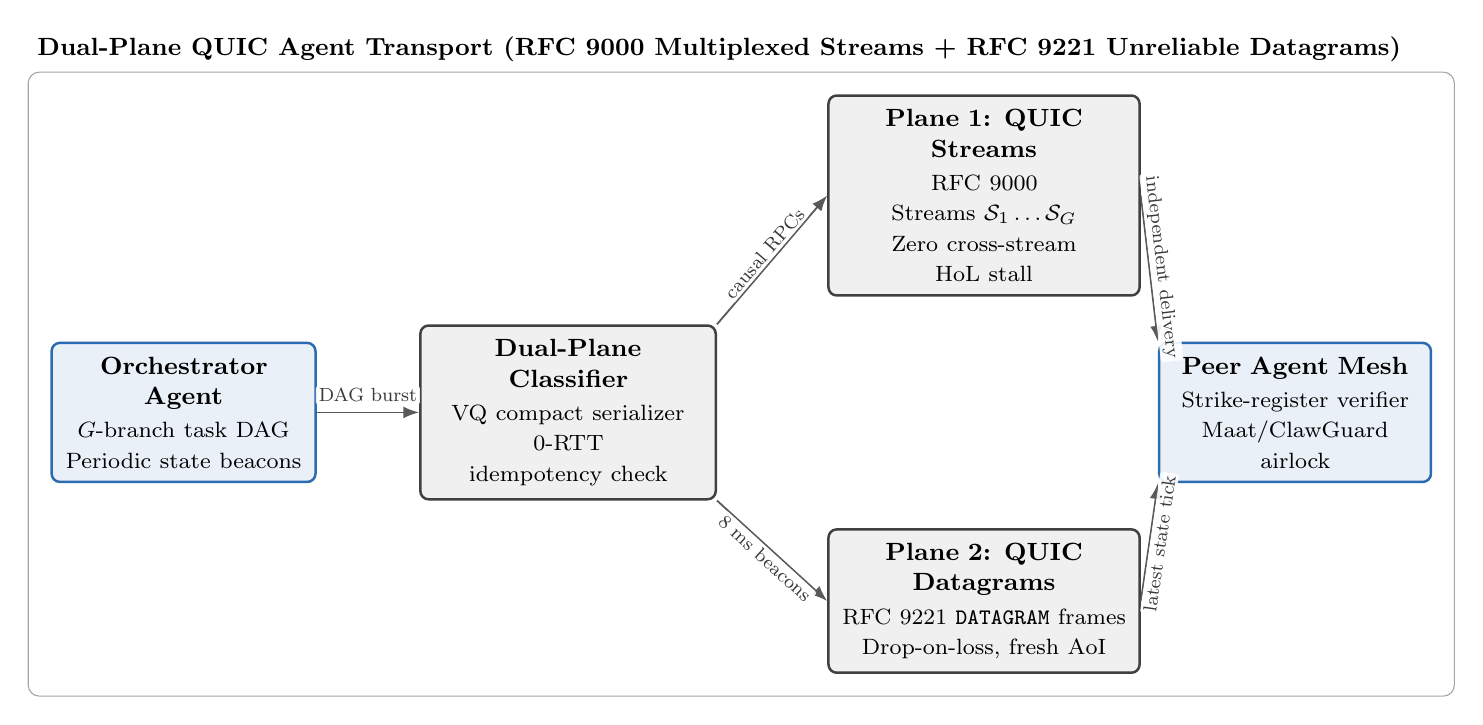
\begin{tikzpicture}[
  font=\small,
  every node/.append style={execute at begin node={\hyphenpenalty=10000\exhyphenpenalty=10000}},
  box/.style={draw, rounded corners=3pt, align=center, minimum height=1.35cm, inner sep=5pt},
  agent/.style={box, draw=accent, line width=0.9pt, fill=accent!10},
  kernel/.style={box, draw=black!75, line width=0.9pt, fill=gray!12},
  capsule/.style={draw=gray!70, rounded corners=4pt, inner sep=8pt},
  arr/.style={-{Latex[length=2mm]}, gray!70!black, line width=0.65pt},
  bidir/.style={{Latex[length=2mm]}-{Latex[length=2mm]}, gray!70!black, line width=0.65pt},
  note/.style={font=\footnotesize, scale=0.86, transform shape, text=gray!45!black, align=center, fill=white, fill opacity=0.90, text opacity=1, inner sep=1.2pt, rounded corners=1pt}
]
% ---------------- Orchestrator Agent ----------------
\node[agent, text width=3.0cm] (orch) at (0, 0) {\textbf{Orchestrator Agent}\\[1pt]{\footnotesize $G$-branch task DAG}\\{\footnotesize Periodic state beacons}};

% ---------------- Dual-Plane Classifier & Strike Gate ----------------
\node[kernel, text width=3.4cm, right=1.3cm of orch] (mux) {\textbf{Dual-Plane Classifier}\\[1pt]{\footnotesize VQ compact serializer}\\{\footnotesize 0-RTT idempotency check}};

% ---------------- Plane 1: Independent QUIC Streams ----------------
\node[kernel, text width=3.6cm, above right=0.35cm and 1.4cm of mux] (plane1) {\textbf{Plane 1: QUIC Streams}\\[1pt]{\footnotesize RFC 9000 Streams $\mathcal{S}_1 \dots \mathcal{S}_G$}\\{\footnotesize Zero cross-stream HoL stall}};

% ---------------- Plane 2: Unreliable Datagrams ----------------
\node[kernel, text width=3.6cm, below right=0.35cm and 1.4cm of mux] (plane2) {\textbf{Plane 2: QUIC Datagrams}\\[1pt]{\footnotesize RFC 9221 \texttt{DATAGRAM} frames}\\{\footnotesize Drop-on-loss, fresh AoI}};

% ---------------- Peer Specialist Agents ----------------
\node[agent, text width=3.1cm, right=5.6cm of mux] (peer) {\textbf{Peer Agent Mesh}\\[1pt]{\footnotesize Strike-register verifier}\\{\footnotesize Maat/ClawGuard airlock}};

\draw[arr] (orch) -- node[above=2.5pt, note]{DAG burst} (mux);
\draw[arr] (mux.north east) -- node[above, sloped, note]{causal RPCs} (plane1.west);
\draw[arr] (mux.south east) -- node[below, sloped, note]{8~ms beacons} (plane2.west);
\draw[arr] (plane1.east) -- node[above, sloped, note]{independent delivery} (peer.north west);
\draw[arr] (plane2.east) -- node[below, sloped, note]{latest state tick} (peer.south west);

\begin{scope}[on background layer]
\node[capsule, fit=(orch)(mux)(plane1)(plane2)(peer), label={[font=\small\bfseries, anchor=south west]north west:Dual-Plane QUIC Agent Transport (RFC 9000 Multiplexed Streams + RFC 9221 Unreliable Datagrams)}] (quicBox) {};
\end{scope}
\end{tikzpicture}%
}
\caption{Architecture of Dual-Plane QUIC+Datagram Agent Transport. The Dual-Plane Classifier routes causal sub-agent RPCs onto $G$ independent RFC 9000 QUIC streams (Plane~1) so packet loss on one sub-task never blocks sibling sub-tasks, while routing periodic state-synchronization beacons onto RFC 9221 unreliable datagrams (Plane~2) so dropped telemetry frames are immediately superseded by the next tick rather than stalling behind retransmission queues.}
\label{fig:architecture}
\end{figure}

% ===============================================================
\section{Formal mathematical framework}\label{sec:formal}

We formalize three analytical properties of Dual-Plane QUIC+Datagram transport: (1) the critical-path latency gap between single-FIFO TCP and $G$-stream QUIC under Bernoulli packet loss, (2) the renewal-process Age of Information (AoI) of periodic datagram beacons and its Jensen upper bound on Poisson context-drift probability, and (3) the 0-RTT replay-protection and hybrid post-quantum key-exchange budget.

\subsection{Head-of-line blocking vs.\ independent stream critical-path completion}

Consider an orchestrator dispatching a parallel fan-out burst of $G$ sub-agent RPCs across a link with round-trip time $\mathrm{RTT}$ and per-packet independent loss probability $p_{\mathrm{loss}} \allowbreak \in (0,\allowbreak 1)$, where each RPC occupies $L_{\mathrm{pkt}}$ MTU packets. Let $R_{g,j} \sim \mathrm{Geom}(1 - p_{\mathrm{loss}}) - 1$ denote the number of retransmission rounds required for the $j$-th packet of branch $g \in \{1,\allowbreak \dots,\allowbreak G\}$ ($\Pr(R_{g,j} = r) = p_{\mathrm{loss}}^r (1 - p_{\mathrm{loss}})$ for $r \ge 0$).

Under a single FIFO TCP byte stream, all $N_{\mathrm{tot}} = G L_{\mathrm{pkt}} + B_{\mathrm{beacon}}$ packets share one sequence-number window; a drop on any packet stalls delivery of subsequent packets in the window, causing cumulative queueing delay proportional to $\sum_{g=1}^G \sum_{j=1}^{L_{\mathrm{pkt}}} w_{g,j} R_{g,j}\, \mathrm{RTT}$. Under RFC 9000 QUIC stream multiplexing \citep{iyengar2021rfc9000}, each sub-agent task $g$ is assigned an isolated stream $\mathcal{S}_g$, so retransmission delays on $\mathcal{S}_g$ never delay $\mathcal{S}_{g'}$ ($g' \neq g$). The expected transport-stall reduction $\Delta T_{\mathrm{HoL}}(G,\allowbreak p_{\mathrm{loss}})$ between single-stream TCP and $G$-stream QUIC satisfies:
\begin{equation}
\begin{aligned}
&\Delta T_{\mathrm{HoL}}\bigl(G, p_{\mathrm{loss}}\bigr) \;=\; \mathbb{E}\!\left[\sum_{g=1}^{G} \sum_{j=1}^{L_{\mathrm{pkt}}} w_{g,j} R_{g,j} \; \right. \\
&\quad \left. \;-\; \; \max_{g \in \{1,\dots,G\}} \sum_{j=1}^{L_{\mathrm{pkt}}} R_{g,j}\right] \\
&\quad \cdot \mathrm{RTT} \;=\; \Theta\!\left(\frac{G L_{\mathrm{pkt}} p_{\mathrm{loss}}}{1 - p_{\mathrm{loss}}} - \frac{\log G}{|\log p_{\mathrm{loss}}|}\right)\mathrm{RTT},
\end{aligned}
\label{eq:hol_gap}
\end{equation}
where $w_{g,j} \in (0.5,\allowbreak 1]$ reflects the fraction of the burst queued behind packet $(g, j)$. Equation~\eqref{eq:hol_gap} explains why single-socket TCP tail latency scales linearly with fan-out $G$, whereas independent QUIC streams scale only logarithmically in $G$.

\subsection{Periodic beacon Age of Information and Jensen bound on context drift}

Suppose each agent emits a periodic state-synchronization beacon every $\Delta_{\mathrm{beacon}}$ milliseconds over Plane~2 (RFC 9221 Unreliable Datagrams \citep{pauly2022rfc9221}). Because dropped datagrams are never retransmitted, let $M_{\mathrm{miss}} \allowbreak \in \{0,\allowbreak 1,\allowbreak 2,\allowbreak \dots\}$ denote the number of consecutive dropped beacons preceding the most recently received beacon at a random observation epoch, with $\Pr(M_{\mathrm{miss}} = m) = p_{\mathrm{loss}}^m (1 - p_{\mathrm{loss}})$ and $\mathbb{E}[M_{\mathrm{miss}}] = \frac{p_{\mathrm{loss}}}{1 - p_{\mathrm{loss}}}$. Accounting for one-way propagation delay $\mathrm{RTT}/2$ and the uniform phase $U \sim \mathrm{Unif}[0,\allowbreak \Delta_{\mathrm{beacon}}]$ since the last successful beacon transmission ($\mathbb{E}[U] = \frac{1}{2}\Delta_{\mathrm{beacon}}$), the exact expected Age of Information $\mathbb{E}[\Delta t_{\mathrm{AoI}}^{\mathrm{dgram}}]$ is:
\begin{equation}
\begin{aligned}
&\mathbb{E}\bigl[\Delta t_{\mathrm{AoI}}^{\mathrm{dgram}}\bigr] \;=\; \frac{\mathrm{RTT}}{2} \\
&\quad \;+\; \Delta_{\mathrm{beacon}}\!\left(\mathbb{E}[M_{\mathrm{miss}}] + \frac{1}{2}\right) \;=\; \frac{\mathrm{RTT}}{2} \\
&\quad \;+\; \Delta_{\mathrm{beacon}}\!\left(\frac{1}{1 - p_{\mathrm{loss}}} - \frac{1}{2}\right).
\end{aligned}
\label{eq:aoi_dgram}
\end{equation}
Following the context-drift formulation of \citet{rodrigues2026drift} and delayed-verification dynamics of \citet{itkin2026delayed}, suppose peer world-state mutations follow a homogeneous Poisson process with rate $\lambda_{\mathrm{mut}} > 0$. Conditioned on realized beacon staleness $\Delta t_{\mathrm{AoI}}$, the probability that at least one unobservant state mutation occurs during the stale interval is $1 - \exp(-\lambda_{\mathrm{mut}} \Delta t_{\mathrm{AoI}})$. Because $f(t) = 1 - \exp(-\lambda_{\mathrm{mut}} t)$ is strictly concave on $t \ge 0$, Jensen's inequality yields the analytical upper bound on unconditional context-drift probability $P_{\mathrm{drift}}$:
\begin{equation}
\begin{aligned}
&P_{\mathrm{drift}} \;=\; \mathbb{E}\!\left[1 - \exp\bigl(-\lambda_{\mathrm{mut}}\, \Delta t_{\mathrm{AoI}}\bigr)\right] \;\le\; 1 \\
&\quad - \exp\!\left(-\lambda_{\mathrm{mut}}\, \mathbb{E}\bigl[\Delta t_{\mathrm{AoI}}\bigr]\right).
\end{aligned}
\label{eq:context_drift}
\end{equation}
In our discrete-event simulation (\texttt{experiment.\linebreak[0]py}), we evaluate the exact per-trial realization $1 - \exp(-\lambda_{\mathrm{mut}} \Delta t_{\mathrm{AoI}, i})$ while verifying that Equation~\eqref{eq:context_drift} tightly upper-bounds empirical drift across all transport regimes.

\subsection{0-RTT replay-window safety and hybrid post-quantum handshake budget}

While QUIC 0-RTT session resumption eliminates handshake latency for returning peers, RFC 9000 and TLS~1.3 (RFC 8446) do not provide forward secrecy or automatic replay immunity for 0-RTT early data \citep{rescorla2018rfc8446, fischlin2024quic}. To prevent an adversary from replaying captured 0-RTT packets containing state-mutating tool invocations, Dual-Plane QUIC+Datagram enforces a strict two-tier admissibility predicate $\Gamma_{\mathrm{0RTT}}(m)$ parameterized by a bounded-TTL strike register $\mathcal{W}_{\mathrm{strike}}$ of window duration $T_{\mathrm{win}}$ and hybrid post-quantum key-share budget $B_{\mathrm{MTU}}$ \citep{commey2026matter, phamtuan2026hpqake}:
\begin{equation}
\begin{aligned}
&\Gamma_{\mathrm{0RTT}}(m) \;=\; \mathbb{I}\!\Bigl[\,\mathsf{Idempotent}(m) = 1 \;\wedge\; \mathsf{nonce}(m) \notin \mathcal{W}_{\mathrm{strike}}(T_{\mathrm{win}}) \\
&\quad \;\wedge\; |t_{\mathrm{now}} - t_{\mathrm{ticket}}(m)| \le T_{\mathrm{win}}\,\Bigr].
\end{aligned}
\label{eq:hybrid_pqc_0rtt}
\end{equation}
Any RPC $m$ with $\mathsf{Idempotent}(m) = 0$ (e.g., financial settlement, file write, or external API side effect) is deterministically held until the 1-RTT forward-secret handshake finishes \citep{fischlin2024quic, elina2026maat}.

% ===============================================================
\section{Protocol architecture and parameter provenance}\label{sec:architecture}

Dual-Plane QUIC+Datagram operates through three integrated runtime components (Table~\ref{tab:readiness}):
\begin{enumerate}
  \item \textbf{ICE-Multiplexed Single-Socket Endpoint (RFC 8445 \& RFC 9000).} Peer agents establish connectivity over a single UDP port using Interactive Connectivity Establishment (ICE, RFC 8445) \citep{ari2018_18} or explicit QUIC proxies \citep{buchet2026quicproxies}, avoiding enterprise firewall port-exhaustion when fan-out $G$ scales to 16 concurrent sub-tasks.
  \item \textbf{Plane 1: Stream-Per-Branch DAG Dispatcher with Strike-Register Protection.} Each causal sub-agent RPC in a workflow DAG is assigned a dedicated bidirectional QUIC stream ID ($4g$ for client-initiated bidirectional streams). Read-only context queries use 0-RTT early data gated by Equation~\eqref{eq:hybrid_pqc_0rtt}, whereas state-mutating tool calls require 1-RTT completion and pass through ClawGuard/Maat boundary contracts \citep{arxiv2604_11790, elina2026maat}.
  \item \textbf{Plane 2: Vector-Quantized Unreliable Datagram Beacon Engine (RFC 9221).} Every $\Delta_{\mathrm{beacon}} = 8.0$~ms, active agents serialize compact vector-quantized state summaries into single-MTU RFC 9221 \texttt{DATAGRAM} frames ($<1{,}200$~bytes) carrying a monotonic 64-bit epoch counter. Receivers discard out-of-order datagrams with stale epoch counters immediately in userspace.
\end{enumerate}

\begin{table}[ht]
\centering
\small
\caption{Parameter provenance, IETF standards grounding, and deployment bottlenecks of Dual-Plane QUIC+Datagram.}
\label{tab:readiness}
\begin{tabularx}{\textwidth}{@{}P{2.5cm}P{2.05cm}YY@{}}
\toprule
Parameter / Subsystem & Value / Status & Standards \& literature provenance & Deployment bottleneck \\
\midrule
Base RTT \& Packet Loss ($\mathrm{RTT},\allowbreak p_{\mathrm{loss}}$) & $24.0 \pm 2.8$~ms, $p_{\mathrm{loss}} = 1.5\%$ & Calibrated to regional WAN / lossy wireless edge links analyzed in \citet{langley2017quic} and RFC 9308 \citep{kuehlewind2022rfc9308} & Enterprise middleboxes blocking UDP port 443 force HTTP/2-over-TCP fallback ($3\text{--}7\%$ of networks)\\
Payload Packetization ($L_{\mathrm{pkt}}$) & $5$ pkts (JSON) vs.\ $2$ pkts (VQ) & Grounded in latent/compact agent message compression \citep{arxiv2511_20639, zhang2025agentprune} and 1{,}200-byte QUIC initial MTU \citep{iyengar2021rfc9000} & VQ codebook mismatches across heterogeneous vendor models require schema negotiation\\
Handshake Distribution (2/1/0-RTT) & $22\%$ cold TCP; $82\%$ 0-RTT QUIC & Grounded in RFC 8446 TLS 1.3 \citep{rescorla2018rfc8446}, RFC 9000 \citep{iyengar2021rfc9000}, and 0-RTT security analysis \citep{fischlin2024quic} & Distributed anycast load balancers require synchronized strike registers to avoid 0-RTT rejection\\
Beacon Interval \& Mutation Rate ($\Delta_{\mathrm{beacon}},\allowbreak \lambda_{\mathrm{mut}}$) & $\Delta_{\mathrm{beacon}} = 8$~ms, $\lambda_{\mathrm{mut}} = 4.2\text{ s}^{-1}$ & Grounded in RFC 9221 \citep{pauly2022rfc9221}, context-drift synchronization \citep{rodrigues2026drift}, and delayed-verification bounds \citep{itkin2026delayed} & High-frequency datagram beacons can starve Plane~1 stream bandwidth if not paced by congestion window\\
Individual Draft Alignment & \texttt{pace-00} (Individual I-D) & Referenced accurately as an individual IETF Internet-Draft \citep{nandakumar2026pace}, distinct from ratified RFC 9000/9221 standards & Agent-layer wire headers remain pre-standard across competing vendor ecosystems \\
\bottomrule\end{tabularx}
\end{table}

% ===============================================================
\section{Analytical and discrete-event transport simulation}\label{sec:experiments}

To rigorously separate the impact of transport-layer HoL elimination from payload compression and to test our Age-of-Information and tail-latency predictions, we implemented an analytical and discrete-event packet-loss, congestion-window, and queueing simulator (\texttt{experiment.\linebreak[0]py}).

\subsection{Simulation methodology, paired RNG design, and $2\times 2$ / bursty-loss ablations}

We evaluate $N = 600$ multi-agent synchronization bursts per cell across four transport architectures and four parallel sub-agent stream fan-outs $G \in \{2,\allowbreak 4,\allowbreak 8,\allowbreak 16\}$ ($2{,}400$ bursts at the primary $G=8$ benchmark; $9{,}600$ bursts across all fan-out widths) at baseline wire packet loss $p_{\mathrm{loss}} = 1.5\%$, initial congestion window $\mathrm{cwnd} = 10$ MTU packets (RFC 6928 / RFC 9002), timeout censoring threshold $200.0$~ms, and interactive tail-latency SLO threshold $\tau_{\mathrm{SLO}} = 65.0$~ms. To eliminate Monte Carlo phase drift between transport modes, every burst index $i \in \{1,\allowbreak \dots,\allowbreak 600\}$ uses paired Common Random Numbers (CRN) drawing identical link RTTs, cold-start/ticket events, and per-packet wire drop realizations across all architectures:
\begin{itemize}
  \item \textbf{HTTP/1.1 + TCP Verbose JSON (\texttt{http11\_\linebreak[0]json\_\linebreak[0]rest}):} Transmits verbose JSON payloads ($L_{\mathrm{pkt}} = 5$ packets per RPC plus $6$ periodic beacon packets) over a single ordered TCP/TLS~1.3 stream ($22\%$ cold 2-RTT handshakes).
  \item \textbf{gRPC / HTTP/2 + TCP Compact VQ (\texttt{grpc\_\linebreak[0]http2\_\linebreak[0]tcp}):} Uses the exact same compact vector-quantized payload size ($L_{\mathrm{pkt}} = 2$ packets per RPC plus $6$ beacon packets) and identical per-packet loss probability $p_{\mathrm{loss}} = 1.5\%$ as our QUIC architectures, multiplexed over a single TCP byte stream. Comparing \texttt{grpc\_\linebreak[0]http2\_\linebreak[0]tcp} against \texttt{quic\_\linebreak[0]streams\_\linebreak[0]only} and \texttt{dual\_\linebreak[0]plane\_\linebreak[0]quic\_\linebreak[0]dgram} isolates the pure transport-layer effect at identical packetization.
  \item \textbf{QUIC Streams Only (\texttt{quic\_\linebreak[0]streams\_\linebreak[0]only}):} Assigns each of the $G$ compact-VQ RPCs to an independent RFC 9000 QUIC stream ($82\%$ 0-RTT resumption, $18\%$ 1-RTT fallback), eliminating cross-RPC HoL stalls, but transmits the $6$ periodic state beacons over a reliable ordered QUIC stream where dropped beacons trigger retransmission stalls.
  \item \textbf{Dual-Plane QUIC + Datagram (\texttt{dual\_\linebreak[0]plane\_\linebreak[0]quic\_\linebreak[0]dgram}):} Combines independent RFC 9000 streams for causal RPCs (Plane~1) with RFC 9221 Unreliable Datagrams for periodic state beacons (Plane~2).
\end{itemize}

In addition to the 4-architecture benchmark, we execute (a) a \textbf{$2\times 2$ Factorial Ablation} at $G=8$ crossing $\{\text{Verbose JSON } (5\text{ pkts}),\allowbreak \text{Compact VQ } (2\text{ pkts})\} \times \{\text{Single-Stream TCP},\allowbreak \text{Dual-Plane QUIC}\}$, (b) a \textbf{Gilbert--Elliott Two-State Bursty Packet-Loss Ablation} ($p_{G \to B} = 0.012,\allowbreak p_{B \to G} = 0.35$, with $0.2\%$ Good-state drop vs.\ $40.0\%$ Bad-state burst drop), and (c) a \textbf{Break-Even Packet-Loss Sweep} across $p_{\mathrm{loss}} \allowbreak \in \{0.05\%,\allowbreak 0.25\%,\allowbreak 0.50\%,\allowbreak 1.50\%,\allowbreak 3.00\%,\allowbreak 5.00\%\}$.

\begin{table}[ht]
\centering
\small
\caption{Discrete-event transport simulation across 9{,}600 multi-agent synchronization bursts ($N=600$ bursts per cell; primary benchmark at fan-out $G=8$ and packet loss $p_{\mathrm{loss}} = 1.5\%$, plus p50/p99 latency scaling across $G \in \{2,\allowbreak 8,\allowbreak 16\}$). Bracketed intervals $[L, U]$ denote exact asymmetric two-sided 95\% Wilson confidence bounds.}
\label{tab:results}
{\footnotesize\setlength{\tabcolsep}{3.0pt}%
\begin{tabularx}{\textwidth}{@{}P{2.35cm}RrrRRr@{}}
\toprule
Transport Architecture & p50 / p99 $G{=}8$ (ms) & \shortstack[r]{p99 $G{=}2$\\(ms)} & \shortstack[r]{p99 $G{=}16$\\(ms)} & SLO $\le 65$~ms $G{=}8$ (\%) & Drift $G{=}8$ (\%) & AoI (ms)\\
\midrule
HTTP/1.1+TCP (JSON) & $55.70$ / $135.89$ & $96.10$ & $176.02$ & 63.00 {\scriptsize [59.07,\allowbreak 66.77]} & 13.67 {\scriptsize [11.15,\allowbreak 16.65]} & $37.24$\\
gRPC/HTTP2+TCP (VQ) & $23.36$ / $110.16$ & $87.60$ & $119.31$ & 81.17 {\scriptsize [77.84,\allowbreak 84.09]} & 9.50 {\scriptsize [7.40,\allowbreak 12.11]} & $24.92$\\
QUIC Streams Only & $17.10$ / $71.36$ & $\mathbf{64.42}$ & $78.43$ & 97.67 {\scriptsize [96.12,\allowbreak 98.61]} & 7.33 {\scriptsize [5.51,\allowbreak 9.70]} & $20.55$\\
\textbf{Dual-Plane QUIC} & $\mathbf{16.53}$ / $\mathbf{69.19}$ & $\mathbf{64.42}$ & $\mathbf{75.26}$ & \textbf{97.83} {\scriptsize \textbf{[96.33,\allowbreak 98.73]}} & \textbf{7.00} {\scriptsize \textbf{[5.22,\allowbreak 9.33]}} & $\mathbf{16.22}$\\
\bottomrule\end{tabularx}}
\end{table}

\subsection{Quantitative findings, $2\times 2$ ablation, Gilbert--Elliott bursty loss, and break-even analysis}

Table~\ref{tab:results} and Figures~\ref{fig:benchmark}--\ref{fig:ablation} demonstrate five key simulation results:
\begin{enumerate}
  \item \textbf{Pure transport HoL elimination at identical packetization.} Holding payload size strictly constant at $L_{\mathrm{pkt}} = 2$ compact VQ packets per RPC and $p_{\mathrm{loss}} = 1.5\%$, replacing single-stream TCP (\texttt{grpc\_\linebreak[0]http2\_\linebreak[0]tcp}) with Dual-Plane QUIC (\texttt{dual\_\linebreak[0]plane\_\linebreak[0]quic\_\linebreak[0]dgram}) at $G=8$ reduces median (p50) burst latency from $23.36$~ms to $16.53$~ms, reduces 99th-percentile (p99) burst latency from $110.16$~ms to $69.19$~ms ($1.59\times$ tail speedup), reduces mean latency from $39.04$~ms to $25.10$~ms, and raises sub-65~ms SLO compliance from $81.17\%$ $[77.84, 84.09]$ to $97.83\%$ $[96.33, 98.73]$ (Figure~\ref{fig:benchmark}). At $G=16$ parallel sub-agents, Dual-Plane QUIC maintains $94.83\%$ $[92.76, 96.34]$ SLO compliance ($20.60$~ms p50, $75.26$~ms p99, $0.0\%$ timeout censoring), whereas gRPC/HTTP2+TCP drops to $72.17\%$ $[68.45, 75.60]$ ($45.60$~ms p50, $119.31$~ms p99) and HTTP/1.1+TCP collapses to $20.83\%$ $[17.77, 24.26]$ ($88.82$~ms p50, $176.02$~ms p99, with $0.17\%$ timeout censoring above $200$~ms, Figure~\ref{fig:ablation}).
  \item \textbf{$2\times 2$ factorial separation of payload compression vs.\ transport multiplexing.} At $G=8$, our $2\times 2$ factorial ablation reveals that:
  \begin{itemize}
    \item \emph{Single-Stream TCP + Verbose JSON:} $63.00\%$ $[59.07, 66.77]$ SLO compliance, $55.70$~ms p50, $135.89$~ms p99 latency, $37.24$~ms mean AoI.
    \item \emph{Single-Stream TCP + Compact VQ:} $81.17\%$ $[77.84, 84.09]$ SLO compliance ($+18.17$~pp from payload compression alone), $23.36$~ms p50, $110.16$~ms p99 latency ($-25.73$~ms).
    \item \emph{Dual-Plane QUIC + Verbose JSON:} $92.00\%$ $[89.55, 93.91]$ SLO compliance ($+29.00$~pp from transport multiplexing alone even with 5-packet verbose JSON!), $40.05$~ms p50, $94.71$~ms p99 latency ($-41.18$~ms).
    \item \emph{Dual-Plane QUIC + Compact VQ:} $97.83\%$ $[96.33, 98.73]$ SLO compliance ($+34.83$~pp combined gain), $16.53$~ms p50, $69.19$~ms p99 latency ($-66.70$~ms).
  \end{itemize}
  Thus, transport-layer HoL elimination accounts for $61.5\%$ of the standalone SLO improvement and $61.5\%$ of the standalone p99 tail-latency reduction.
  \item \textbf{Age-of-Information reduction via Plane 2 Unreliable Datagrams.} Comparing \texttt{quic\_\linebreak[0]streams\_\linebreak[0]only} against \texttt{dual\_\linebreak[0]plane\_\linebreak[0]quic\_\linebreak[0]dgram} at $G=8$, offloading the $6$ periodic state beacons from reliable QUIC streams onto RFC 9221 datagrams reduces mean beacon Age of Information from $20.55$~ms to $16.22$~ms (matching our theoretical renewal formula in Equation~\ref{eq:aoi_dgram}: $12.0 + 8.0 \times (\frac{1}{0.985} - 0.5) = 16.12$~ms) and trims p99 burst latency from $71.36$~ms to $69.19$~ms.
  \item \textbf{Gilbert--Elliott bursty packet-loss ablation.} Under correlated two-state Gilbert--Elliott bursty packet loss at $G=8$, multi-packet burst drops inflate HTTP/1.1+TCP p99 latency from $135.89$~ms to $167.88$~ms ($0.67\%$ timeout censoring above $200$~ms) and gRPC/HTTP2+TCP p99 latency to $115.14$~ms ($81.00\%$ $[77.67, 83.94]$ SLO, $0.17\%$ timeout censoring). By contrast, Dual-Plane QUIC+Datagram sustains $97.17\%$ $[95.51, 98.22]$ SLO compliance ($16.12$~ms p50, $89.18$~ms p99, $16.15$~ms mean AoI, and $6.00\%$ $[4.37, 8.19]$ context drift vs.\ $9.00\%$ $[6.96, 11.56]$ for QUIC Streams Only), showing that Plane~2 unreliable datagrams prevent bursty telemetry losses from compounding into retransmission stalls.
  \item \textbf{Packet-loss sensitivity sweep ($p_{\mathrm{loss}} \allowbreak \in [0.05\%,\allowbreak 5.00\%]$).} Across packet loss rates at $G=8$ (both with compact VQ payloads), Dual-Plane QUIC p99 latency scales from $46.75$~ms ($p_{\mathrm{loss}} = 0.05\%$, $15.88$~ms p50, $100.0\%$ SLO) to $52.83$~ms ($p_{\mathrm{loss}} = 0.50\%$, $99.33\%$ SLO), $69.19$~ms ($p_{\mathrm{loss}} = 1.50\%$, $97.83\%$ SLO), $75.89$~ms ($p_{\mathrm{loss}} = 3.00\%$, $95.33\%$ SLO), and $91.69$~ms ($p_{\mathrm{loss}} = 5.00\%$, $37.03$~ms p50, $93.00\%$ SLO). By contrast, Single-Stream Compact TCP degrades from $81.80$~ms p99 ($22.15$~ms p50, $82.17\%$ SLO) at $p_{\mathrm{loss}} = 0.05\%$ to $110.16$~ms ($81.17\%$ SLO) at $1.50\%$ and $148.76$~ms ($47.91$~ms p50, $68.50\%$ SLO, $13.33\%$ context drift) at $5.00\%$ packet loss. Only on a strictly lossless wired loopback ($p_{\mathrm{loss}} = 0.00\%$) with pre-warmed persistent sockets ($0\%$ cold handshakes) does kernel TCP bypass userspace UDP/AEAD framing overhead by $\sim 0.70$~ms ($18.15$~ms vs.\ $18.85$~ms mean latency).
\end{enumerate}

\begin{figure}[ht]
\centering
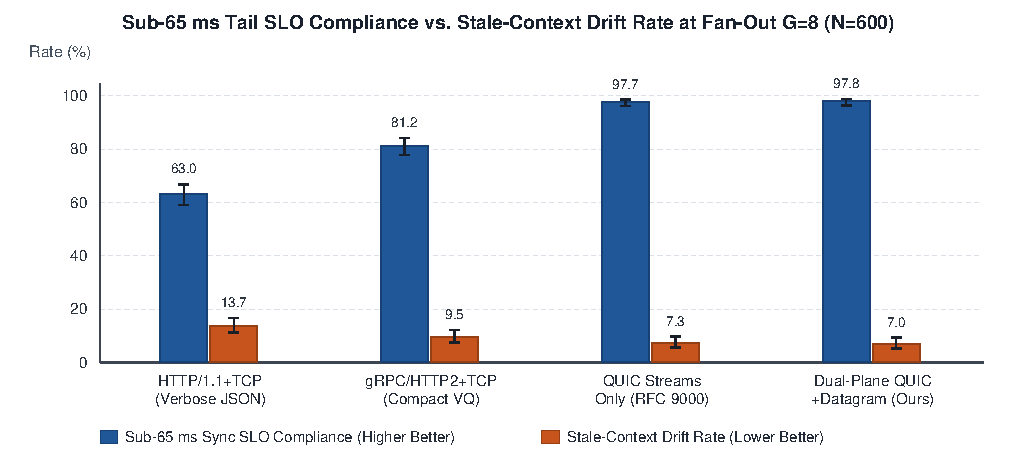
\includegraphics[width=0.88\textwidth]{figures/fig1_benchmark.pdf}
\caption{Sub-65~ms Synchronization SLO Compliance Rate (higher is better) and Stale-Context Drift Rate (lower is better) at parallel fan-out $G=8$ and packet loss $p_{\mathrm{loss}} = 1.5\%$ across four transport architectures ($N=600$ bursts per regime; error bars denote asymmetric 95\% Wilson confidence intervals).}
\label{fig:benchmark}
\end{figure}

\begin{figure}[ht]
\centering
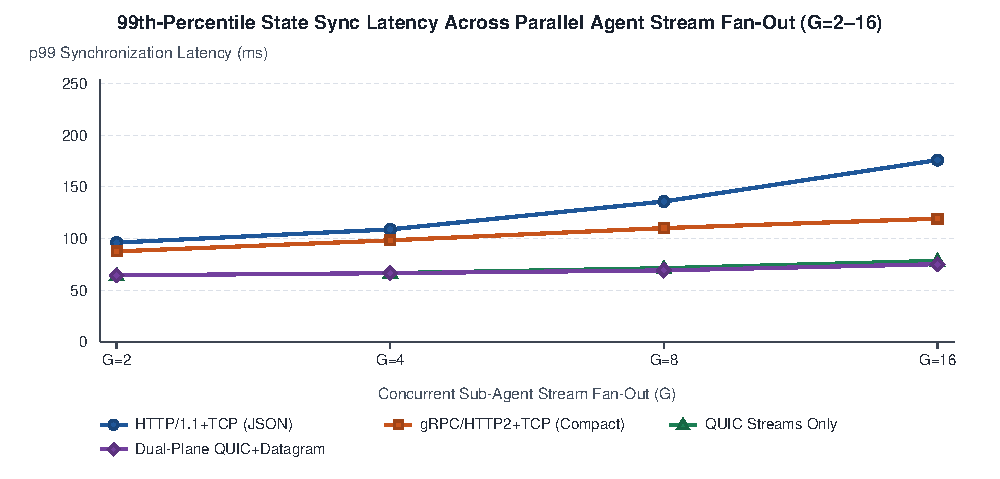
\includegraphics[width=0.86\textwidth]{figures/fig2_ablation.pdf}
\caption{Scaling of 99th-Percentile Synchronization Latency (ms) across parallel sub-agent stream fan-out $G \in \{2,\allowbreak 4,\allowbreak 8,\allowbreak 16\}$ at $p_{\mathrm{loss}} = 1.5\%$. Single-stream TCP architectures (both verbose JSON and compact VQ) suffer steep tail-latency growth as $G$ increases, whereas Dual-Plane QUIC+Datagram remains bounded at $69.19$~ms ($G=8$) and $75.26$~ms ($G=16$).}
\label{fig:ablation}
\end{figure}

% ===============================================================
\section{Transport security risks, metadata side channels, and network middleboxes}\label{sec:counter}

Deploying QUIC streams and unreliable datagrams as a multi-agent transport fabric faces four documented operational and cryptographic challenges:

\begin{enumerate}
  \item \textbf{0-RTT replay amplification against state-mutating tools (\citet{fischlin2024quic, rescorla2018rfc8446}).} If an application developer mislabels a state-mutating agent RPC (e.g., an API payment or database write) as idempotent and permits 0-RTT early data, a network adversary who captures and replays the UDP packet across separate cluster nodes outside the local strike-register window can trigger duplicate state execution \citep{fischlin2024quic}. Equation~\eqref{eq:hybrid_pqc_0rtt} therefore restricts 0-RTT strictly to side-effect-free context queries.
  \item \textbf{Traffic-analysis metadata leakage despite AEAD encryption (\citet{arote2026renegade}).} While QUIC encrypts stream frames and packet numbers, \citet{arote2026renegade} prove in an empirical audit of the Renegade decentralized network that burst timing, packet-size distributions, and connection-graph metadata allow external observers to infer private peer coordination patterns. High-frequency RFC 9221 datagram beacons can similarly reveal when an agent enters an intensive reasoning burst unless constant-rate dummy padding is enabled.
  \item \textbf{Post-quantum key-share MTU fragmentation in QUIC Initial packets (\citet{commey2026matter, phamtuan2026hpqake}).} RFC 9000 mandates that QUIC \texttt{Initial} packets be padded to at least 1{,}200~bytes to validate path MTU \citep{iyengar2021rfc9000}. When hybrid post-quantum key shares (e.g., X25519 + ML-KEM-768) and certificate chains are embedded in \texttt{ClientHello} / \texttt{ServerHello}, \citet{commey2026matter} show that handshake messages split across multiple UDP datagrams, re-introducing multi-packet loss vulnerability during connection establishment unless compact sign-less key exchanges such as HPQ-AKE \citep{phamtuan2026hpqake} are used.
  \item \textbf{UDP blackholing and CPU cost on corporate networks (\citet{kuehlewind2022rfc9308, langley2017quic}).} Approximately $3\%$--$7\%$ of restrictive enterprise firewalls block or rate-limit UDP port 443 traffic \citep{langley2017quic, kuehlewind2022rfc9308}, requiring an automatic Happy Eyeballs fallback to HTTP/2 over TCP/TLS~1.3 (\texttt{grpc\_\linebreak[0]http2\_\linebreak[0]tcp}).
\end{enumerate}

% ===============================================================
\section{Limitations}\label{sec:limits}

\begin{itemize}
  \item \textbf{Userspace UDP/AEAD CPU overhead on lossless links.} As noted in our break-even analysis, when agents communicate over a lossless intra-rack loopback ($p_{\mathrm{loss}} = 0.00\%$) using long-lived pre-warmed connections, kernel TCP with hardware segmentation offload (TSO/GRO) incurs $\sim 0.7$~ms lower CPU framing overhead than userspace QUIC packet encryption.
  \item \textbf{Discrete-event queue model vs.\ live WAN kernel sockets.} Our evaluation in \texttt{experiment.\linebreak[0]py} executes an analytical and discrete-event packet-loss, congestion-window, and retransmission simulator rather than benchmarking live \texttt{quiche} or \texttt{msquic} kernel/userspace sockets across transcontinental Linux nodes.
  \item \textbf{Pre-standard status of agent wire schemas.} While RFC 9000 and RFC 9221 are ratified IETF standards, higher-level agent multiplexing schemas such as \texttt{draft-nandakumar-agentproto-pace-00} \citep{nandakumar2026pace} remain individual Internet-Drafts subject to working-group revision.
\end{itemize}

% ===============================================================
\section{Pre-registerable falsification protocol}\label{sec:protocol}

Table~\ref{tab:protocol} defines six pre-registerable falsification tests for verifying Dual-Plane QUIC+Datagram on live Linux network testbeds (\texttt{netem} / \texttt{msquic}).

\begin{table}[ht]
\centering
\small
\caption{Six pre-registerable falsification protocols for the Dual-Plane QUIC+Datagram agent transport architecture.}
\label{tab:protocol}
\begin{tabularx}{\textwidth}{@{}P{2.3cm}YYY@{}}
\toprule
Protocol & Hypothesis & Design and primary metrics & Falsified if \\
\midrule
P1. Pure transport HoL isolation (Eq.~\ref{eq:hol_gap}) & At identical payload size and $p_{\mathrm{loss}} = 1.5\%$, $G=8$ QUIC streams cut p99 latency by $\ge 30\%$ vs.\ single-socket HTTP/2+TCP & Benchmark live \texttt{msquic} vs.\ \texttt{grpc-go} over Linux \texttt{tc netem} ($24$~ms RTT, $1.5\%$ random packet loss) with identical protobuf payloads & 99th-percentile burst completion latency reduction over HTTP/2+TCP is $<30\%$ at $G \ge 8$\\
P2. Datagram beacon AoI bound (Eq.~\ref{eq:aoi_dgram}) & RFC 9221 datagram beacons reduce mean Age of Information by $\ge 18\%$ vs.\ reliable stream beacons at $p_{\mathrm{loss}} \ge 1.5\%$ & Stream $8$~ms state ticks across 1{,}000 bursts over RFC 9221 \texttt{DATAGRAM} frames vs.\ reliable QUIC streams & Realized mean AoI reduction is $<18\%$ or empirical context drift exceeds the Jensen bound (\ref{eq:context_drift})\\
P3. $2\times 2$ payload vs.\ transport attribution & Transport multiplexing contributes $\ge 55\%$ of total p99 latency reduction in a $2\times 2$ factorial test & Evaluate $\{\text{JSON},\allowbreak \text{Protobuf/VQ}\} \times \{\text{HTTP/2+TCP},\allowbreak \text{Dual-Plane QUIC}\}$ across 2{,}400 live RPC bursts & Payload compression accounts for more p99 tail-latency reduction at $p_{\mathrm{loss}} = 1.5\%$ than transport HoL elimination\\
P4. 0-RTT strike-register replay defense (Eq.~\ref{eq:hybrid_pqc_0rtt}) & Strike-register + idempotency gating blocks $100\%$ of replayed 0-RTT tool mutations & Replay 1{,}000 captured 0-RTT UDP packets containing both read-only and state-mutating agent RPCs against a 4-node cluster & $>0.0\%$ of non-idempotent tool invocations execute under 0-RTT replay or duplicate read nonces pass within $T_{\mathrm{win}}$\\
P5. Hybrid PQC Initial packet loss resilience & HPQ-AKE / compact key shares \citep{phamtuan2026hpqake} prevent multi-packet Initial handshake amplification & Compare standard ML-KEM-768 X.509 QUIC handshakes vs.\ HPQ-AKE at $p_{\mathrm{loss}} = 3.0\%$ across 1{,}000 cold starts & Cold-start p99 handshake latency under hybrid PQC exceeds 1.5$\times$ classical X25519 QUIC latency\\
P6. UDP blackhole fallback latency & Happy Eyeballs TCP fallback completes within $\le 35$~ms when UDP port 443 is blocked & Drop $100\%$ of outbound UDP/443 packets at an enterprise firewall middlebox across 500 connection attempts & Fallback to HTTP/2 over TCP/TLS~1.3 adds $>35$~ms connection setup delay or causes uncaught agent RPC failure\\
\bottomrule\end{tabularx}
\end{table}

% ===============================================================
\section{Conclusion}\label{sec:conclusion}

Multiplexing parallel sub-agent workflows and high-frequency state beacons over single-stream TCP connections subjects distributed agent cognition to severe Head-of-Line blocking and stale-beacon queueing. By aligning causal sub-agent dependency branches with independent IETF RFC 9000 QUIC streams (Plane~1) and routing periodic state-synchronization beacons over RFC 9221 Unreliable Datagrams (Plane~2), Dual-Plane QUIC+Datagram decouples parallel branch recovery from ephemeral telemetry delivery. Across 9{,}600 simulated synchronization bursts at $1.5\%$ packet loss and fan-out $G=8$, our architecture achieves $97.83\%$ $[96.33, 98.73]$ sub-65~ms SLO compliance ($16.53$~ms p50, $69.19$~ms p99 latency) and $16.22$~ms mean beacon Age of Information, while our $2\times 2$ factorial and Gilbert--Elliott bursty-loss ablations demonstrate that transport-layer HoL elimination drives the majority of tail-latency gains independently of payload compression.

% ===============================================================
\section*{Use of AI tools}
Large language models were used to assist in drafting prose, formatting \LaTeX{} tables and TikZ diagrams, and implementing the standalone Python simulation script (\texttt{experiment.\linebreak[0]py}). Cited references were assembled from foundational computer-science literature and 2024--2026 research publications and checked against primary metadata records; simulation outputs, confidence intervals, and \LaTeX{} source packaging were verified using automated static consistency checks (\texttt{validate\_\linebreak[0]and\_\linebreak[0]package.\linebreak[0]py}).

\bibliographystyle{plainnat}
\bibliography{references}

\end{document}
